\documentclass[a4paper, twoside, 12pt]{report}

\usepackage{titlesec}
\usepackage{polski}
\usepackage[english, polish]{babel}
\usepackage{graphicx}
\usepackage[hidelinks]{hyperref}
\usepackage{pdfpages}
\graphicspath{ {./images/} }
\usepackage[utf8]{inputenc}
\usepackage[margin=25mm]{geometry}
\usepackage{indentfirst}
\linespread{1}
\titleformat*{\section}{\fontsize{14pt}{2}\bfseries}
\titleformat*{\subsection}{\fontsize{13pt}{2}\bfseries}
\titleformat*{\subsubsection}{\fontsize{13pt}{2}\bfseries}
\usepackage[T1]{fontenc}
% \usepackage{tgtermes}

\newenvironment{abstractpage}
  {\vspace*{\fill}\thispagestyle{empty}}
    {\vfill}
    \renewenvironment{abstract}[1]
      {\bigskip\selectlanguage{#1}%
             \begin{center}\bfseries\abstractname\end{center}}
           {\par\bigskip}

\begin{document}

% 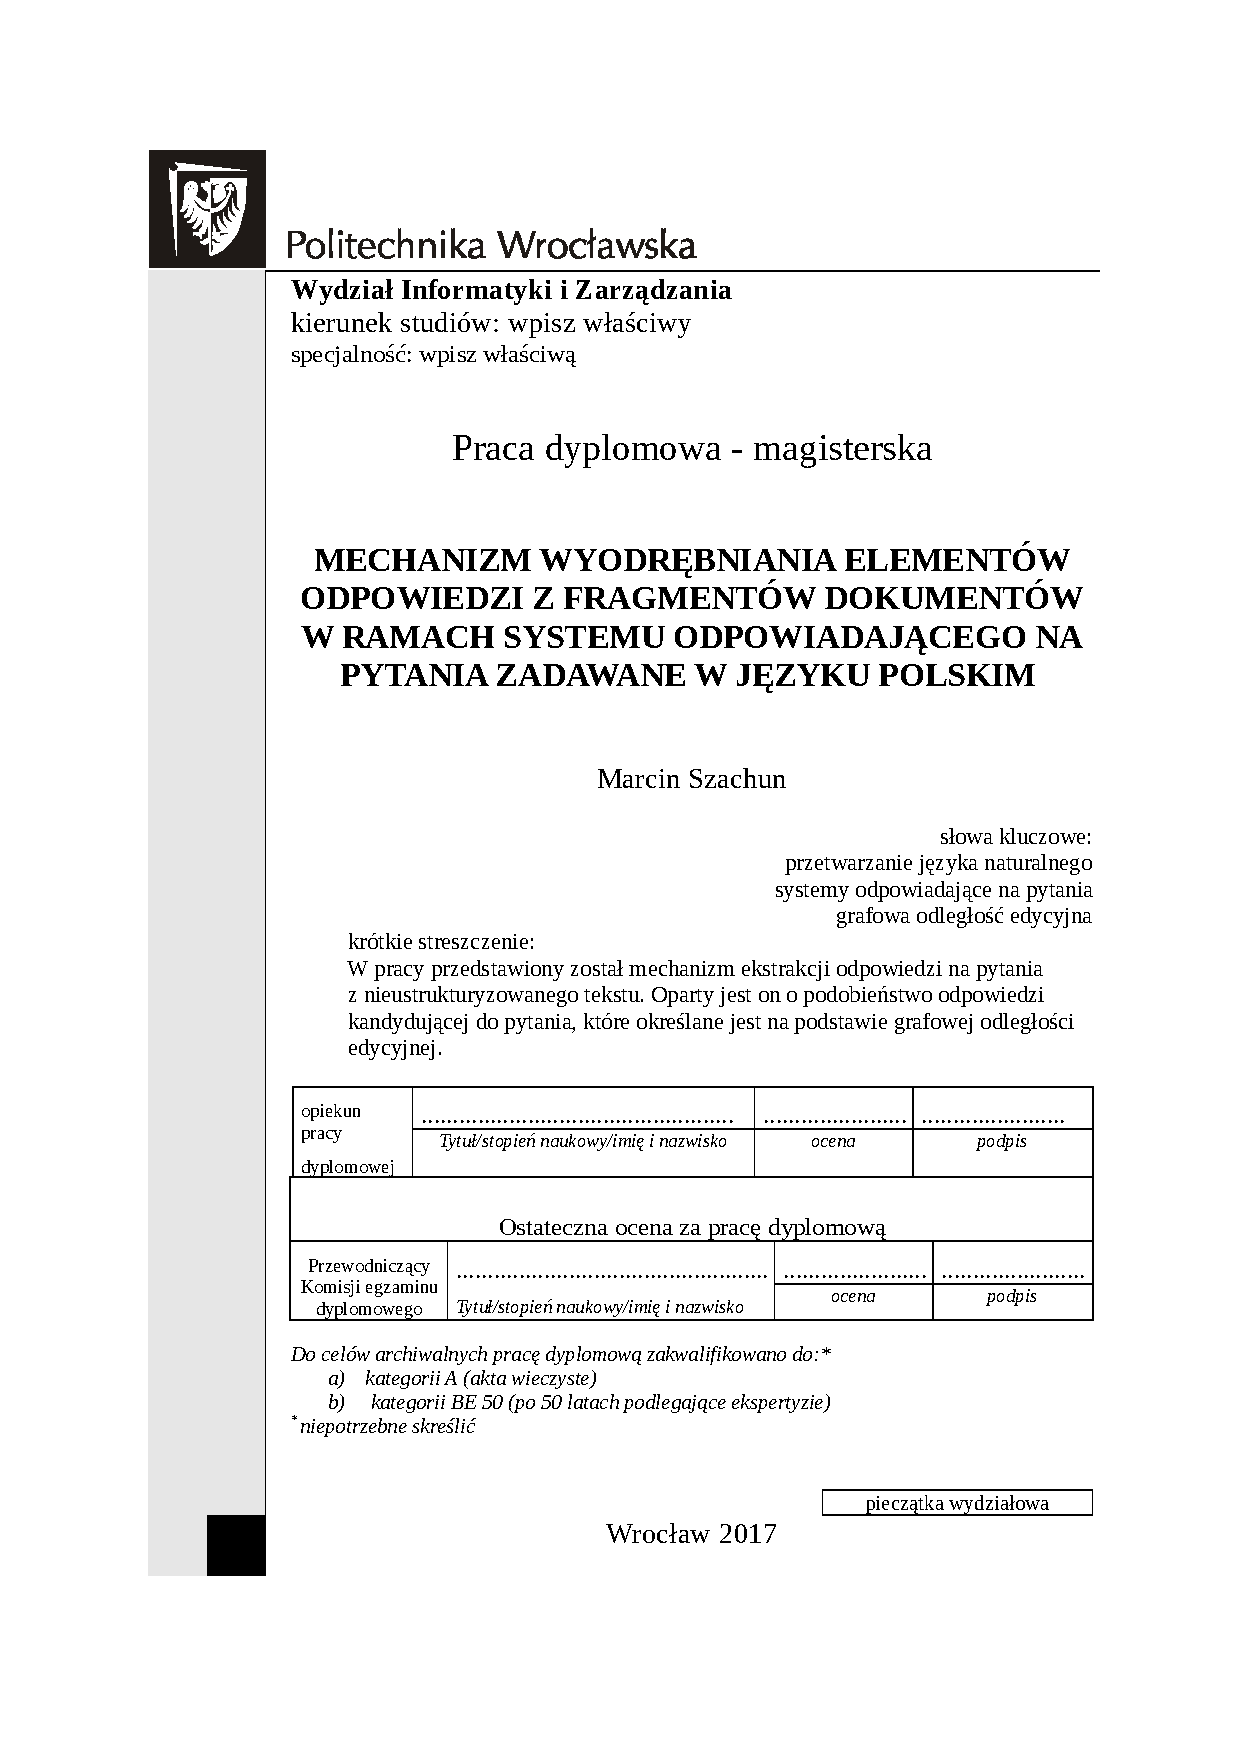
\includepdf{stronatytulowa.pdf}


\begin{abstractpage}
\begin{abstract}{polish}
    W dzisiejszych czasach Internet pełen jest informacji na praktycznie dowolny temat. Wraz ze wzrastającą ilością
    dostępnych informacji, coraz ważniejsze staje się opracowanie mechanizmów pozwalających znaleźć informacje
    interesujące użytkownika. Tradycyjnie w tym celu wykorzystywane były wyszukiwarki internetowe. Niestety
    języki zapytań używane przez wyszukiwarki internetowe powodują, że wyrażenie precyzyjnej potrzeby informacyjnej
    przez użytkownika jest trudne, a niekiedy niemożliwe. Jednym z proponowanych rozwiązań tego problemu są systemy
    odpowiadające na pytania, w których zapytania formułowane są w formie pytań w języku naturalnym. Niniejsza
    praca zawiera krótkie przedstawienie dziedziny Question Answering, zajmującej się tworzeniem tego typu systemów,
    wraz z opisem systemu "Borsuk" stworzonego na Politechnice Wrocławskiej.
    W głównej części pracy opisana została propozycja nowego mechanizmu ekstrakcji odpowiedzi z fragmentów dokumentów,
    opartego na zmodyfikowanej odległości edycyjnej jako miary podobieństwa między pytaniem a zdaniami mogącymi zawierać
    odpowiedź. Modyfikacja polega na dynamicznym przypisywaniu kosztu operacjom edycji w zależność od słowa. Przeprowadzone
    zostały badania pozwalające optymalnie dobrać wartości tych kosztów. Po zaimplementowaniu tego mechanizmu w systemie "Borsuk",
    wykonane zostały też badania mające na celu porównanie precyzji i dokładności odpowiadania na pytania przed i po
    zastosowaniu opisywanego mechanizmu.
\end{abstract}

\begin{abstract}{english}
    Nowadays the Internet is full of information on almost every topic. With growing amount of available information,
    providing ways to find specific information that user wants is becoming more and more important. Traditionally
    search engines were intended for that purpose. Unfortunately query languages used by search engines are sometimes
    insufficient for expressing user's infomation needs. One of proposed solutions are question answering systems, in which
    queries are formulated using natural language. This thesis contains quick overview of question answering discipline,
    which is concerned with build such systems and description of "Borsuk" system, created by Wrocław University of Technology.
    In main part, new answer extraction mechanism is presented. It is based on using modified tree edit distance as a measure of
    similarity question and sentences that ma contain answer. Modification lies in dynamically assing cost to edit operations
    based on word. Research was conducted to find out optimal cost for operations. Furthermore after implementing this
    mechanism in "Borsuk" question answering system, additional research was conducted to compare precision and accuracy
    of question answering before and after using described mechanism
\end{abstract}
\end{abstractpage}

\tableofcontents

\listoffigures

\chapter{Cel i~zakres pracy}
    Celem niniejszej pracy jest przedstawienie mechanizmu rozszerzającego system odpowiadający na pytania ,,Borsuk''
    pod względem dokładności udzielanych odpowiedzi. Zastosowany mechanizm wykorzystuje odległość edycyjną jako miarę
    podobieństwa między pytaniem a zdaniami zawierającymi odpowiedzi. W~ramach tego celu zostaną wykonane:
    \begin{itemize}
        \item prezentacja i ogólna charakterystyka dziedziny Question Answering wraz z przedstawieniem podstawowych
            pojęć,
        \item przedstawienie przykładowych, innych niż zaproponowany w~pracy,
            sposobów ekstrakcji odpowiedzi na pytania z fragmentów dokumentów,
        \item zaprezentowanie mechanizmu ekstrakcji odpowiedzi z wykorzystaniem odległości edycyjnej między grafami
            reprezentującymi pytanie oraz zdania kandydujące na odpowiedzi,
        \item przeprowadzenie badań pozwalających na dobranie optymalnych parametrów działania opisywanego
            mechanizmu ekstrakcji odpowiedzi wraz z analizą wniosków z nich płynących,
       \item zaprezentowanie sprawozdania z przebiegu oraz wyników badań porównujących precyzję i dokładność
           odpowiadania na pytania przez system "Borsuk" przed i po implementacji opisanego mechanizmu ekstrakcji
           odpowiedzi.
       \item przeanalizowanie możliwych sposobów kontynuacji prac nad udoskonaleniem przedstawionego mechanizmu

    \end{itemize}

\chapter{Wstęp teoretyczny}
\clearpage
\addcontentsline{toc}{chapter}{Bibliografia}
\bibliographystyle{plain}
%\bibliography{bibliografia}


\end{document}
